\chapter[Referencial teórico]{Referencial teórico}

Este capítulo apresenta o referencial teórico que fornece a base para o desenvolvimento deste trabalho. Abordamos os conceitos de prototipação e design de serviço, trazendo como foco a etapa da prototipação no ciclo de vida do serviço. O segundo tópico de discussão são as principais técnicas e ferramentas de prototipação disponíveis no mercado. Também é abordado o papel do cliente na prototipagem de serviços, visando entender a importância da participação do mesmo na elaboração do protótipo. Por último, uma contextualização no geral da prototipagem no design de serviço, como a mesma se relaciona com outras etapas mencionando onde ela se situa.  

\section{Prototipação}

A prototipação é um processo chave no que se diz respeito ao desenvolvimento de novas soluções, produtos ou sistemas. Nesse sentido modelos preliminares ou representações de ideias são criados como teste para conceitos e hipóteses. A definição da palavra protótipo, de forma generalista é "A primeira forma" \cite{Blomkvist2011existing}.

Os protótipos manifestam conceitos, ideias ou palpites sobre quais boas soluções podem ser. Esta é uma maneira de mostrar o conceito e garantir que todos os envolvidos tenham a chance de entendê-lo. \cite{Blomkvist2014}

Portanto, a função principal de um protótipo é testar ideias de forma prática e sólida, ajudando a refinar e validar conceitos antes do investimento na solução ou produto final, que na maioria dos casos é muito mais alto. Outro ponto não menos importante, é que ao criar protótipos, existe a possibilidade de obter feedbacks valiosos de clientes, usuários e as partes interessadas, trazendo uma segurança a mais que o produto ou solução desenvolvida esteja alinhada com as expectativas e necessidades.

\subsection{Objetivos}

Seguindo as discussões expostas anteriormente, é possível traçar alguns objetivos principais da prototipação, sendo eles:

\begin{itemize}
	\item \textbf{Visualização de conceitos:} Fazer com que uma ideia ou conceito tenha seu entendimento facilitado entre membros da equipe e partes interessadas.
	
	\item \textbf{Experimentação:} Permitir a experimentação com diversos tipos de soluções e abordagens, fazendo com que problemas e limitações sejam identificados no ínicio.
	
	\item \textbf{Obtenção de feedback:} Coletar opiniões, sugestões e críticas dos usuários e stakeholders para ajudar a melhorar e ajustar as soluções em andamento.
\end{itemize}

Esses objetivos mostram como a prototipação tem um papel fundamental no desenvolvimento de soluções eficazes e de acordo com as necessidades do usuário por exemplo. A visualização de conceitos traz um entendimento mútuo entre todos que estão envolvidos no projeto, resultando na redução de compreensões distintas ao longo do processo. Já a experimentação traz maiores garantias para que, no momento da implementação final, seja um processo mais tranquilo. Além disso, a obtenção de feedbacks, ao fazer com que os usuários e stakeholders atuem ativamente, torna o produto ou serviço mais relevante e funcional.

\subsection{Benefícios}

\section{Introdução ao Design de Serviços}

\subsection{Definição}

A definição de design de serviço pode ser algo muito subjetivo, uma vez que muitos autores definem de uma maneira diferente, e além disso, é uma área holística, abrangendo muitos processos, atividades e mentalidades. Porém, ainda sim é possível traçar um paralelo entre as definições mais aceitas.

O design de serviço ajuda as organizações a enxergarem seus serviços pela perspectiva do cliente. É uma abordagem para projetar serviços que equilibra as necessidades do cliente e as necessidades do negócio, buscando criar experiências de serviço fluidas e de qualidade. O design de serviço se ancora no design thinking e oferece um processo criativo e centrado no ser humano para a melhoria de serviços e o projeto de novos serviços. Por meio de métodos colaborativos que envolvem clientes e equipes de serviço, ele ajuda as organizações a obterem uma compreensão verdadeira e completa de seus serviços, possibilitando melhorias holísticas e significativas. \cite{Stickdorn2019}

Neste sentido, entre os profissionais do design de serviço, ainda existem muitas discordâncias em relação à diferenças entre áreas próximas. Assim, existem os defensores de que deve-se separar design de serviço de design de experiência, design thinking, experiência do usuário holística, entre outros. Mas também existem aqueles que acreditam que são áreas muito semelhantes, portanto creem que nomenclaturas não devem ser levadas tão a sério.

\subsection{O que design de serviço não é}

Por ser uma área ampla, é importante delimitar o escopo sobre o que não está englobado no design de serviço, para que não tenha nenhuma confusão nesse sentido. Logo abaixo são citados alguns tópicos que não são cobertos pelo design de serviço:

\begin{itemize}
	\item \textbf{Não é estética}: Designers de serviço se preocupam muito mais com funcionamento e criação de valor, do que se o mesmo tem uma boa aparência ou não.
	
	\item \textbf{Não é "atendimento ao cliente"}: É justamente o que ele visa evitar, uma vez que, quanto melhor e mais intuitivo o serviço é, de menos suporte o cliente irá necessitar, logo diminuindo a questão de atendimento ao cliente.
	
	\item \textbf{Não é "recuperação de serviço"}: Muito pelo contrário, o design de serviço deve ser utilizado durante o processo de criação, e não quando o produto/serviço já deu errado e precisa de alguma salvação milagrosa.
	
\end{itemize}

\subsection{Princípios do design de serviço}

Existe uma discussão sobre o que são os princípios de fato do design de serviço. Isso ocorre devido à diversos fatores, mas o principal deles, foi a reunião de cinco princípios fundamentais no livro "Isto é design de serviço", lançado em 2010. Esses princípios foram fortemente difundidos, porém se fez necessário uma revisão dos mesmos, uma vez que alguns ficaram um pouco defasados com o tempo, então neste ponto acaba havendo um descompasso entre os princípios presentes nesse livro e os princípios mais condizentes com a realidade. Esses eram os princípios:

\begin{itemize}
	\item \textbf{Centrado no usuário}: serviços devem ser testados através do olhar do cliente.
	\item \textbf{Cocriativo}: todos stakeholders devem ser incluídos no processo do desenho do serviço.
	\item \textbf{Sequenciado}: o serviço deve ser visualizado como uma sequência de ações inter-relacionadas.
	\item \textbf{Evidente}: serviços intangíveis devem ser visualizados por meio de suas evidências físicas.
	\item \textbf{Holístico}: todo o ambiente de um serviço deve ser levado em consideração.
\end{itemize}
	
Alguns dos princípios necessitaram de uma breve modificação, sendo de uma palavra ou outra, já outros, tiveram que passar por uma reformulação mais significativa.

O primeiro, ao ser nomeado como \textbf{"centrado no usuário"} traz uma interpretação de que pode-se excluir alguns grupos que também interagiam com o sistema, como a equipe interna por exemplo. Logo no lugar de \textbf{"usuário"}, fez mais sentido a utilização de \textbf{"ser humano"} para assim englobar de forma mais adequada todos os grupos.

O segundo, ao ser chamado de \textbf{"Cocriativo"} é o resultado da união de dois conceitos, \textbf{"cocriação"} e \textbf{"codesign"}. O primeiro trabalha no sentido de valor gerado por serviços, já o segundo traz uma ideia do "processo de criação feito por um grupo de pessoas, normalmente vindas de diferentes contextos."\cite{Stickdorn2019} Porém, com o tempo, o foco foi mais direcionado para esse segundo conceito.

O terceiro, com a nomenclatura de \textbf{"Sequenciado"} faz referência à importância da relação entre os vários momentos de contato com o serviço. Neste caso, a mudança necessária foi somente para o melhor entendimento do princípio, não mudando nada no seu significado original, uma vez que a palavra "sequenciado" não é comum no cotidiano das pessoas. 

O quarto, titulado de \textbf{"Evidente"} reconhece a intangibilidade de algumas partes do serviço, destacando sempre o valor do serviço em si, mesmo que não exista uma maneira clara e tangível de avaliar essa importância.

O quinto, conceituado de \textbf{"Holístico"}, foi chamado assim por basicamente reunir muitos conceitos em uma palavra só. Ao defender essa reunião de conceitos como "a relevância de todos os nossos sentidos para uma experiência de serviço; outro é a ampla variedade de jornadas individuais que um serviço pode gerar; e o último trata da relevância do design de serviço para a identidade corporativa e para as metas de uma organização."\cite{Stickdorn2019} 

Outro ponto importante, é que nesses cinco princípios originais, não houve ênfase em uma característica fundamental do design de serviço, a \textbf{iteração}. A iteração se diz respeito à começar com tentativas que não visam a perfeição, mas sim a simplicidade e com base nisso, naturalmente haverão falhas, e com essas falhas, lições devem ser aprendidas para que as próximas tentativas sejam melhores, ou seja, aprender com as falhas.

Com base nesses pontos de revisão e melhoria, os seguintes novos princípios de design de serviço surgiram: \cite{Stickdorn2019}

\begin{itemize}
	\item \textbf{Centrado no ser humano}: considera a experiência de todas as pessoas afetadas pelo serviço.
	\item \textbf{Colaborativo}: stakeholders advindos de contextos e funções variados devem se envolver ativamente no processo de desenho de um serviço.
	\item \textbf{Iterativo}: o design de serviço é uma abordagem exploratória, adaptativa e experimental, que promove a iteração do protótipo de um serviço rumo a sua implementação.
	\item \textbf{Sequencial}:o serviço deve ser visualizado e regido como uma sequência de ações inter-relacionadas.
	\item \textbf{Real}: as necessidades do usuário devem ser pesquisadas no mundo real, as ideias devem ser prototipadas no mundo real e os valores intangíveis devem ser postos em evidência por meio de uma realidade física ou digital.
	\item \textbf{Holístico}:  devem ser consideradas, de modo sustentável, as necessidades de todos os stakeholders ao longo do serviço e a interação com todas as facetas do negócio.
\end{itemize}

Resumidamente, o design de serviço "é uma abordagem centrada no ser humano, colaborativa, interdisciplinar, iterativa, que utiliza pesquisa, prototipação e um conjunto de atividades e ferramentas de visualização de fácil entendimento para criar e orquestrar experiências que atendam às necessidades do negócio, do usuário e dos stakeholders do serviço."\cite{Stickdorn2019}

\begin{figure}[h]
	\centering % para centralizarmos a figura
	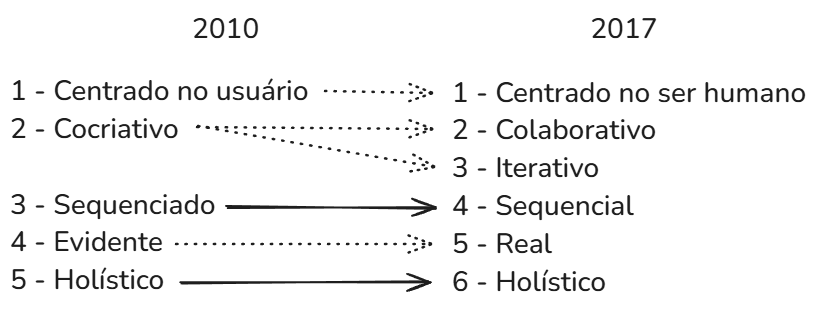
\includegraphics[width=15cm]{figuras/principios.png} % leia abaixo
	\caption{Transição dos princípios do design de serviço}
	Fonte: Livro - Isto é design de serviço na prática
	\label{figura:qualquernome}
\end{figure}

\section{Relação da prototipação com o design de serviço}

%Não esquecer de falar de prototipação como um processo iterativo
% A prototipação no design de serviços é um processo essencialmente iterativo. Isso significa que, em vez de criar um único protótipo final, a ideia é desenvolver várias versões de um protótipo, refinando-o a cada iteração com base nos testes e feedback obtidos. A iteração é a sequência de testes e aprimoramentos sucessivos de um protótipo, permitindo que ele evolua gradualmente até atender aos requisitos esperados \cite{Christie2012}.

%\section{Técnicas e ferramentas} -> Vai ser resultado

%\section{Papel do cliente} -> Vai ser resultado

\section{Contexto}
